\documentclass[a4paper]{article}
\usepackage[a4paper,margin=1in,landscape]{geometry}
\usepackage[utf8]{inputenc}
\usepackage[T1]{fontenc}
\usepackage{longtable}
\usepackage[table,svgnames]{xcolor}
\usepackage{colortbl}
\usepackage{pgfplots}
\pgfplotsset{width=10cm,compat=1.14}
\usepgfplotslibrary{dateplot}
\usetikzlibrary{plotmarks}
\usepackage{booktabs}
\usepackage{array}
\usepackage{eurosym}
\usepackage{forest}
\usepackage{listings}
\usepackage{multicol}
\usepackage{fancyhdr}
\pagestyle{fancy}
\lfoot{Section \leftmark}
\cfoot{}
\rfoot{\thepage}
\rhead{Generated: \today}
\chead{}
\lhead{Scheduling Report}
\usepackage{hyperref}
\title{Scheduling Report}
\author{L. O'Toole and H. Simonis}
\date{Report Generated on \today}

\begin{document}
\maketitle
\definecolor{wipcolor}{RGB}{128,128,128}
\definecolor{downcolor}{RGB}{255,0,0}
\definecolor{latecolor}{RGB}{255,0,0}
\definecolor{makespancolor}{RGB}{255,0,0}
\definecolor{resourcecolor}{RGB}{0,0,255}
\definecolor{jobcolor}{RGB}{0,255,0}
\definecolor{stagecolor0}{RGB}{240,163,255}
\definecolor{stagecolor1}{RGB}{0,117,220}
\definecolor{stagecolor2}{RGB}{153,63,0}
\definecolor{stagecolor3}{RGB}{76,0,92}
\definecolor{stagecolor4}{RGB}{25,25,25}
\definecolor{stagecolor5}{RGB}{0,92,49}
\definecolor{stagecolor6}{RGB}{43,206,72}
\definecolor{stagecolor7}{RGB}{255,204,153}
\section{Introduction}

\begin{table}[htbp]
\caption{Problem}
\centering
\begin{tabular}{llrrrrrrrr} \toprule
Name &Label &\shortstack{Timepoints\\as\\Date} &\shortstack{Nr\\Products} &\shortstack{Nr\\Process} &\shortstack{Nr\\Disjunctive\\Resources} &\shortstack{Nr\\Cumulative\\Resources} &\shortstack{Nr\\Orders} &\shortstack{Nr\\Jobs} &\shortstack{Nr\\Tasks} \\ \midrule
Generated&&true&10&10&8&1&50&50&200\\ 
\bottomrule
\end{tabular}
\end{table}

\section{Orders}

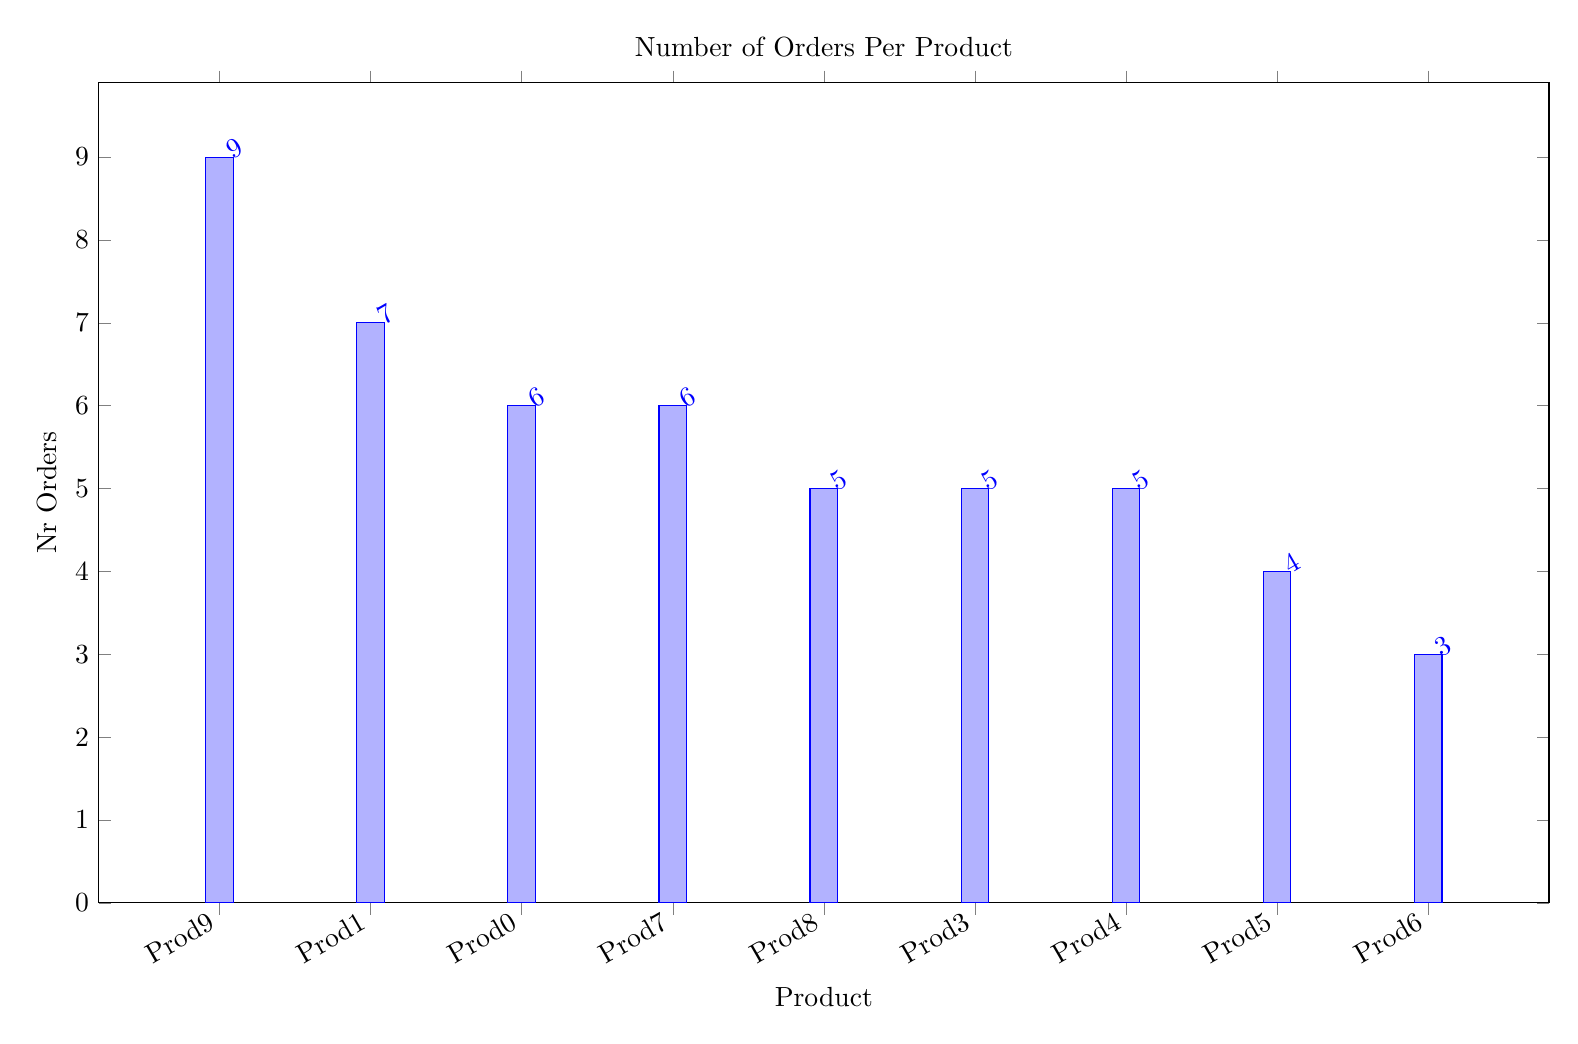
\begin{tikzpicture}
\begin{axis}[title=Number of Orders Per Product,xlabel=Product,ylabel=Nr Orders,ymin=0,width=20cm,height=12cm,ybar,symbolic x coords={Prod9,Prod1,Prod0,Prod7,Prod8,Prod3,Prod4,Prod5,Prod6},
    xtick=data,
    nodes near coords, 
    nodes near coords align={rotate=30,anchor=west},
    x tick label style={rotate=30,anchor=east},
]
\addplot+[] coordinates {
(Prod9,9.000000)
(Prod1,7.000000)
(Prod0,6.000000)
(Prod7,6.000000)
(Prod8,5.000000)
(Prod3,5.000000)
(Prod4,5.000000)
(Prod5,4.000000)
(Prod6,3.000000)
};
\end{axis}
\end{tikzpicture}

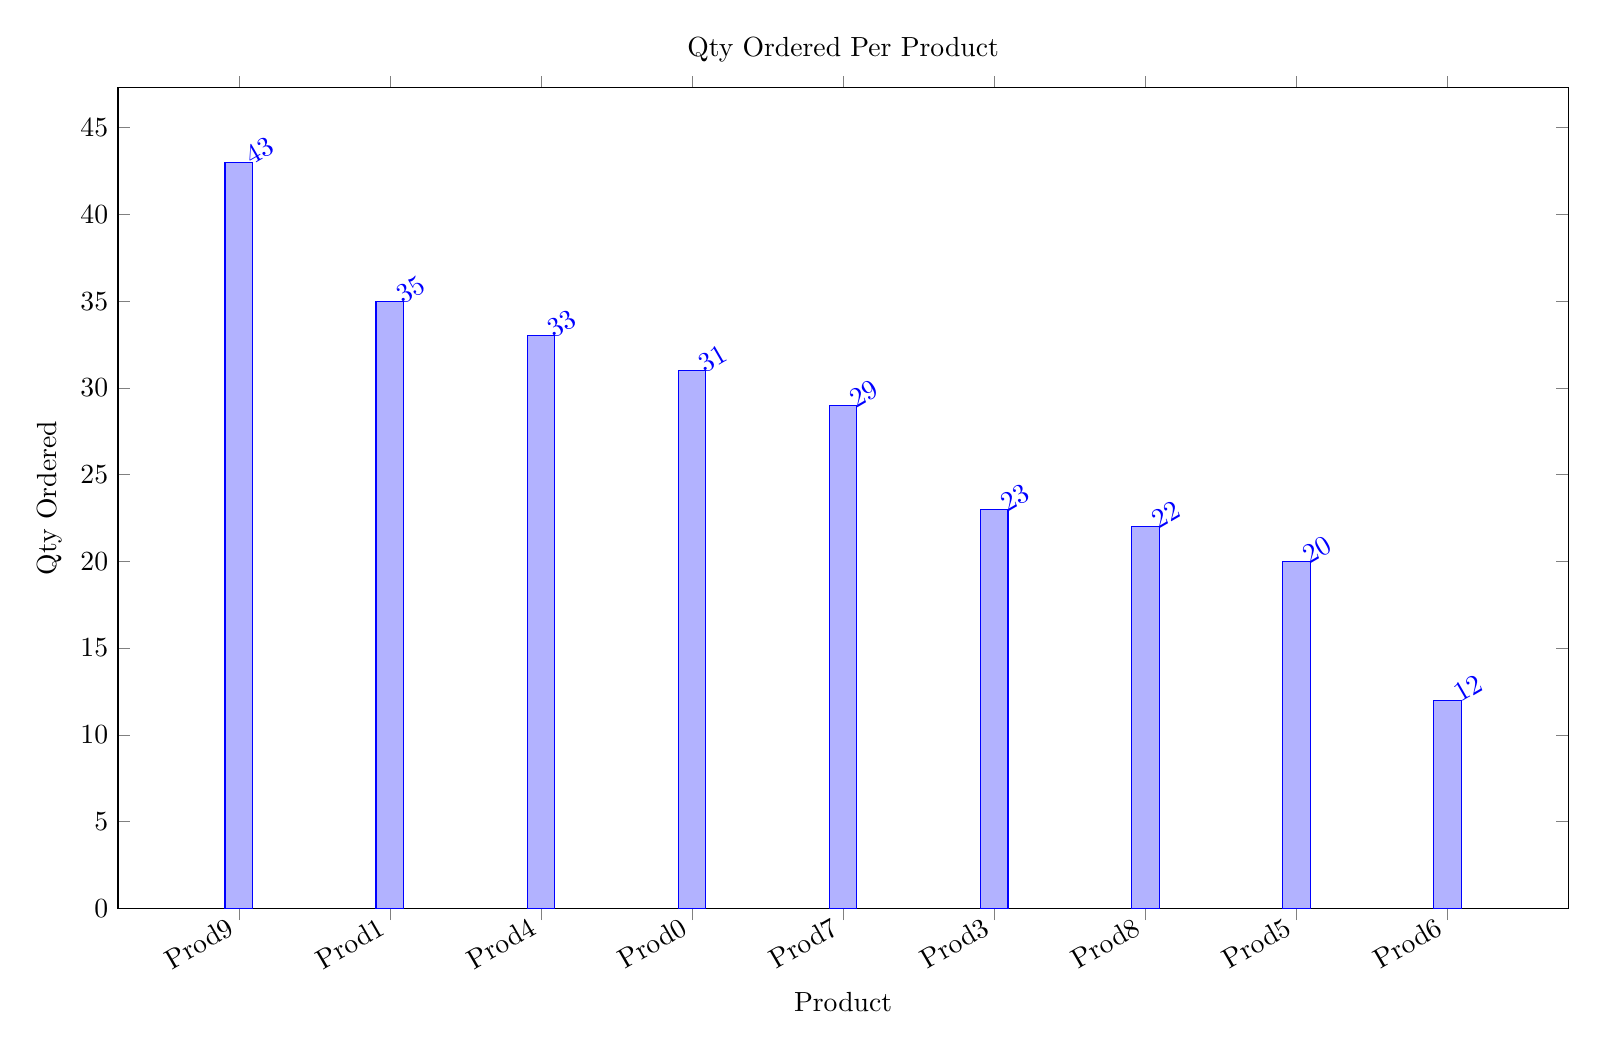
\begin{tikzpicture}
\begin{axis}[title=Qty Ordered Per Product,xlabel=Product,ylabel=Qty Ordered,ymin=0,width=20cm,height=12cm,ybar,symbolic x coords={Prod9,Prod1,Prod4,Prod0,Prod7,Prod3,Prod8,Prod5,Prod6},
    xtick=data,
    nodes near coords, 
    nodes near coords align={rotate=30,anchor=west},
    x tick label style={rotate=30,anchor=east},
]
\addplot+[] coordinates {
(Prod9,43.000000)
(Prod1,35.000000)
(Prod4,33.000000)
(Prod0,31.000000)
(Prod7,29.000000)
(Prod3,23.000000)
(Prod8,22.000000)
(Prod5,20.000000)
(Prod6,12.000000)
};
\end{axis}
\end{tikzpicture}

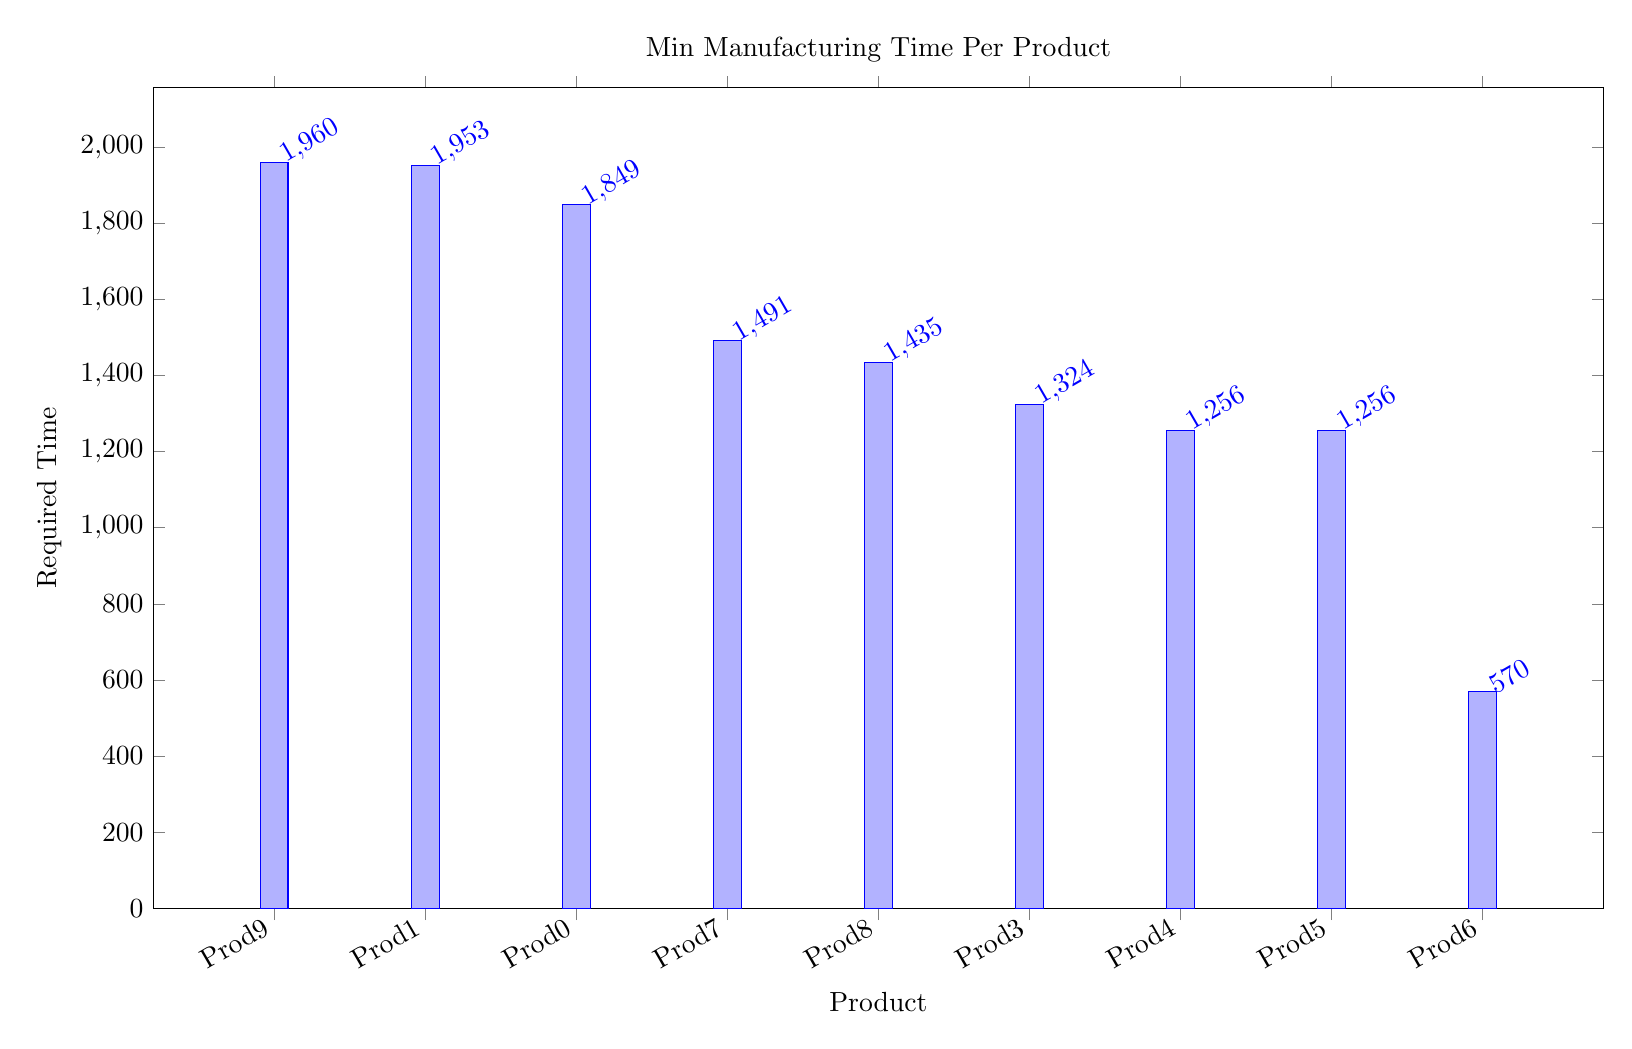
\begin{tikzpicture}
\begin{axis}[title=Min Manufacturing Time Per Product,xlabel=Product,ylabel=Required Time,ymin=0,width=20cm,height=12cm,ybar,symbolic x coords={Prod9,Prod1,Prod0,Prod7,Prod8,Prod3,Prod4,Prod5,Prod6},
    xtick=data,
    nodes near coords, 
    nodes near coords align={rotate=30,anchor=west},
    x tick label style={rotate=30,anchor=east},
]
\addplot+[] coordinates {
(Prod9,1960.000000)
(Prod1,1953.000000)
(Prod0,1849.000000)
(Prod7,1491.000000)
(Prod8,1435.000000)
(Prod3,1324.000000)
(Prod4,1256.000000)
(Prod5,1256.000000)
(Prod6,570.000000)
};
\end{axis}
\end{tikzpicture}

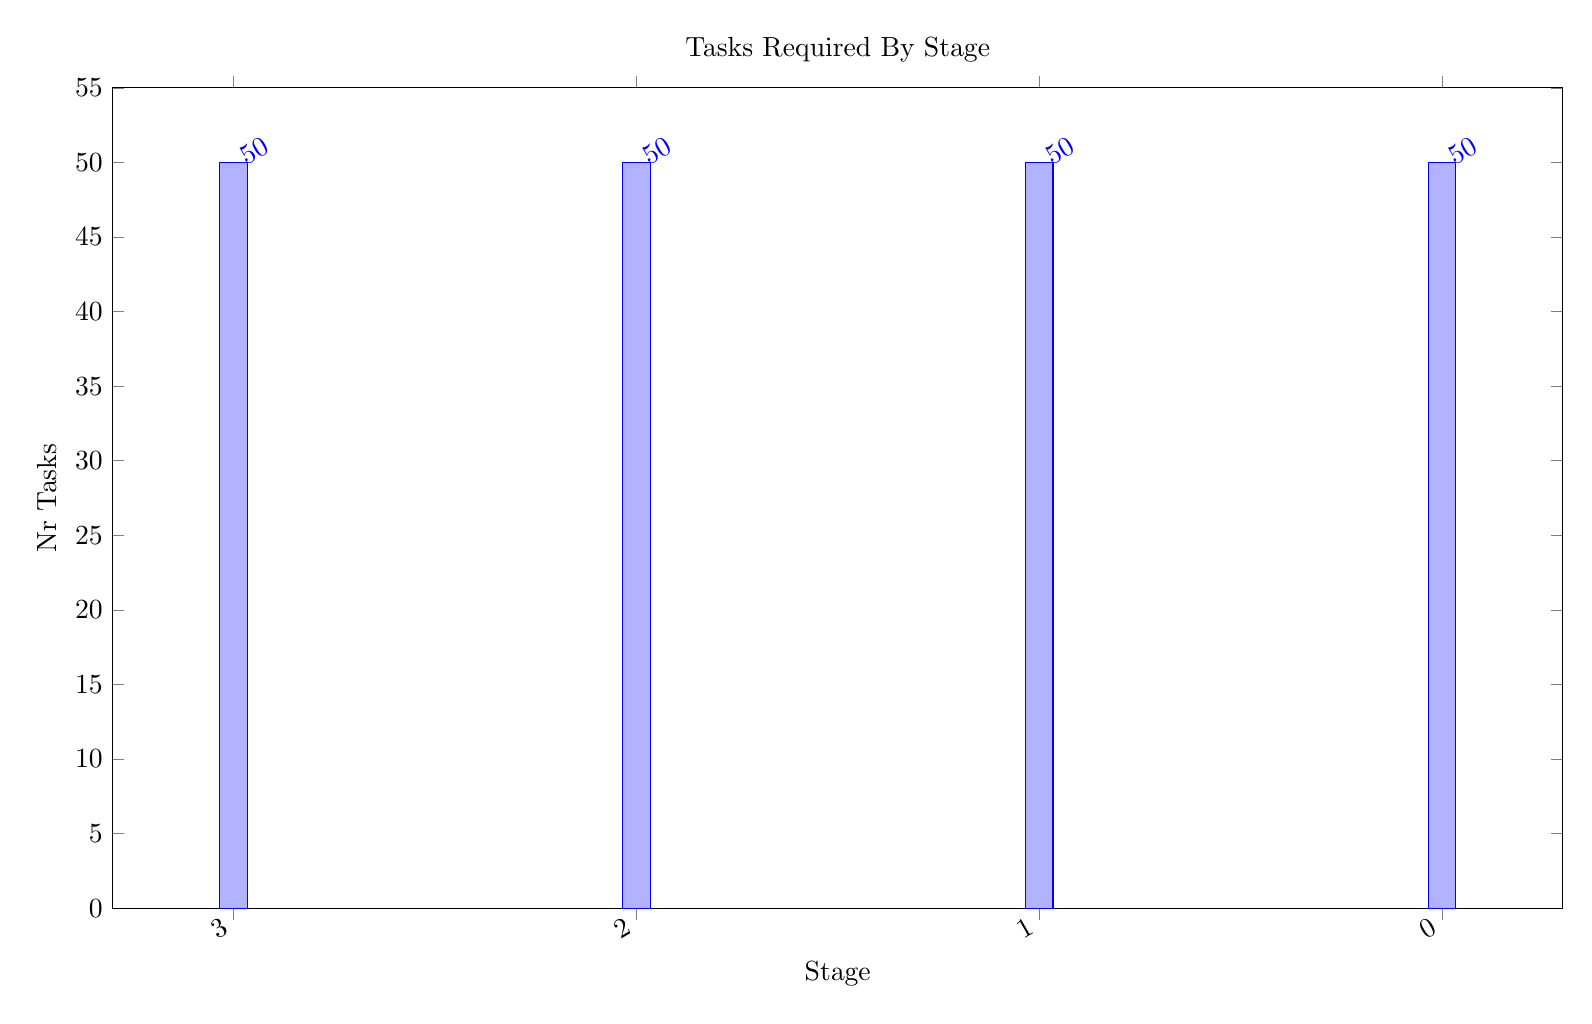
\begin{tikzpicture}
\begin{axis}[title=Tasks Required By Stage,xlabel=Stage,ylabel=Nr Tasks,ymin=0,width=20cm,height=12cm,ybar,symbolic x coords={3,2,1,0},
    xtick=data,
    nodes near coords, 
    nodes near coords align={rotate=30,anchor=west},
    x tick label style={rotate=30,anchor=east},
]
\addplot+[] coordinates {
(3,50.000000)
(2,50.000000)
(1,50.000000)
(0,50.000000)
};
\end{axis}
\end{tikzpicture}

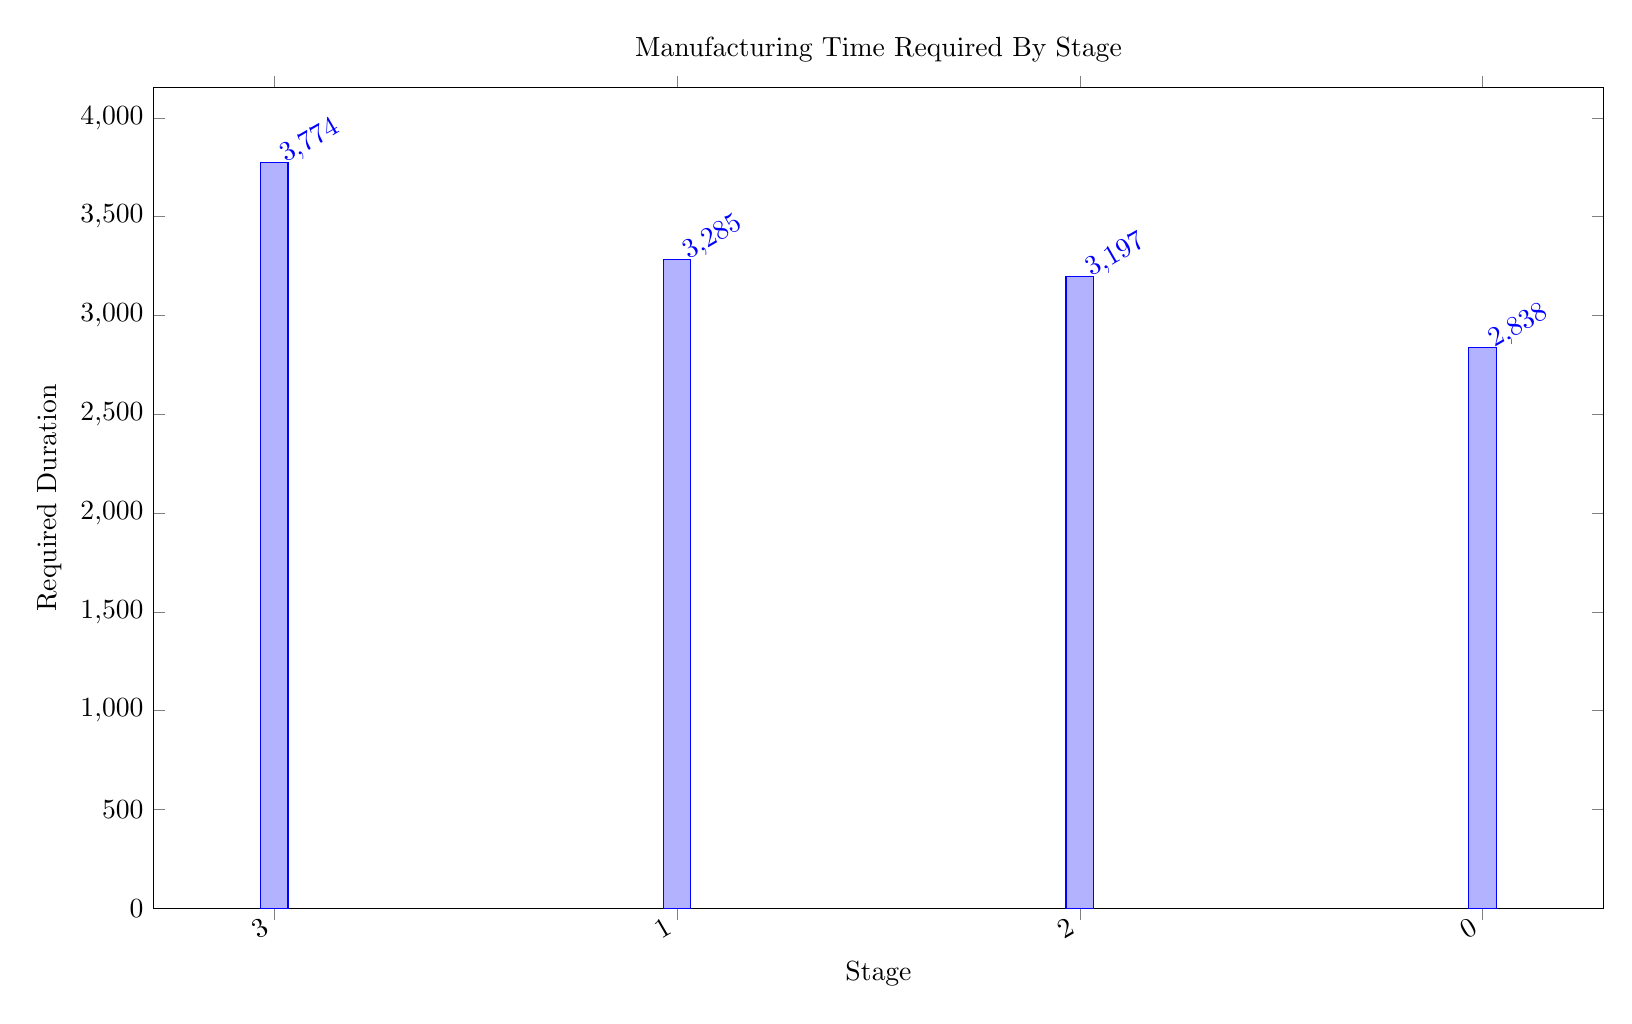
\begin{tikzpicture}
\begin{axis}[title=Manufacturing Time Required By Stage,xlabel=Stage,ylabel=Required Duration,ymin=0,width=20cm,height=12cm,ybar,symbolic x coords={3,1,2,0},
    xtick=data,
    nodes near coords, 
    nodes near coords align={rotate=30,anchor=west},
    x tick label style={rotate=30,anchor=east},
]
\addplot+[] coordinates {
(3,3774.000000)
(1,3285.000000)
(2,3197.000000)
(0,2838.000000)
};
\end{axis}
\end{tikzpicture}

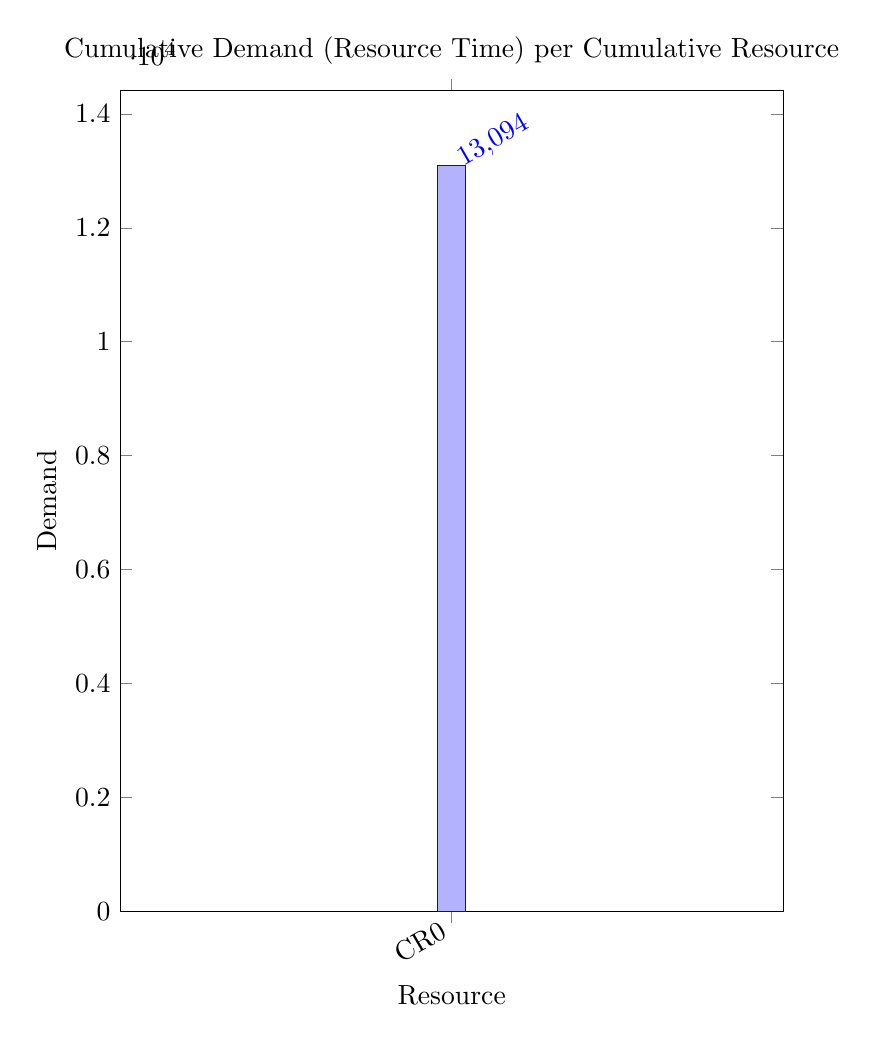
\begin{tikzpicture}
\begin{axis}[title=Cumulative Demand (Resource Time) per Cumulative Resource,xlabel=Resource,ylabel=Demand,ymin=0,
width=10cm,height=12cm,ybar,
symbolic x coords={CR0},
    xtick=data,nodes near coords, nodes near coords align={rotate=30),anchor=west},x tick label style={rotate=30),anchor=east}]
\addplot+[] coordinates {
(CR0,13094.000000)
};
\end{axis}
\end{tikzpicture}

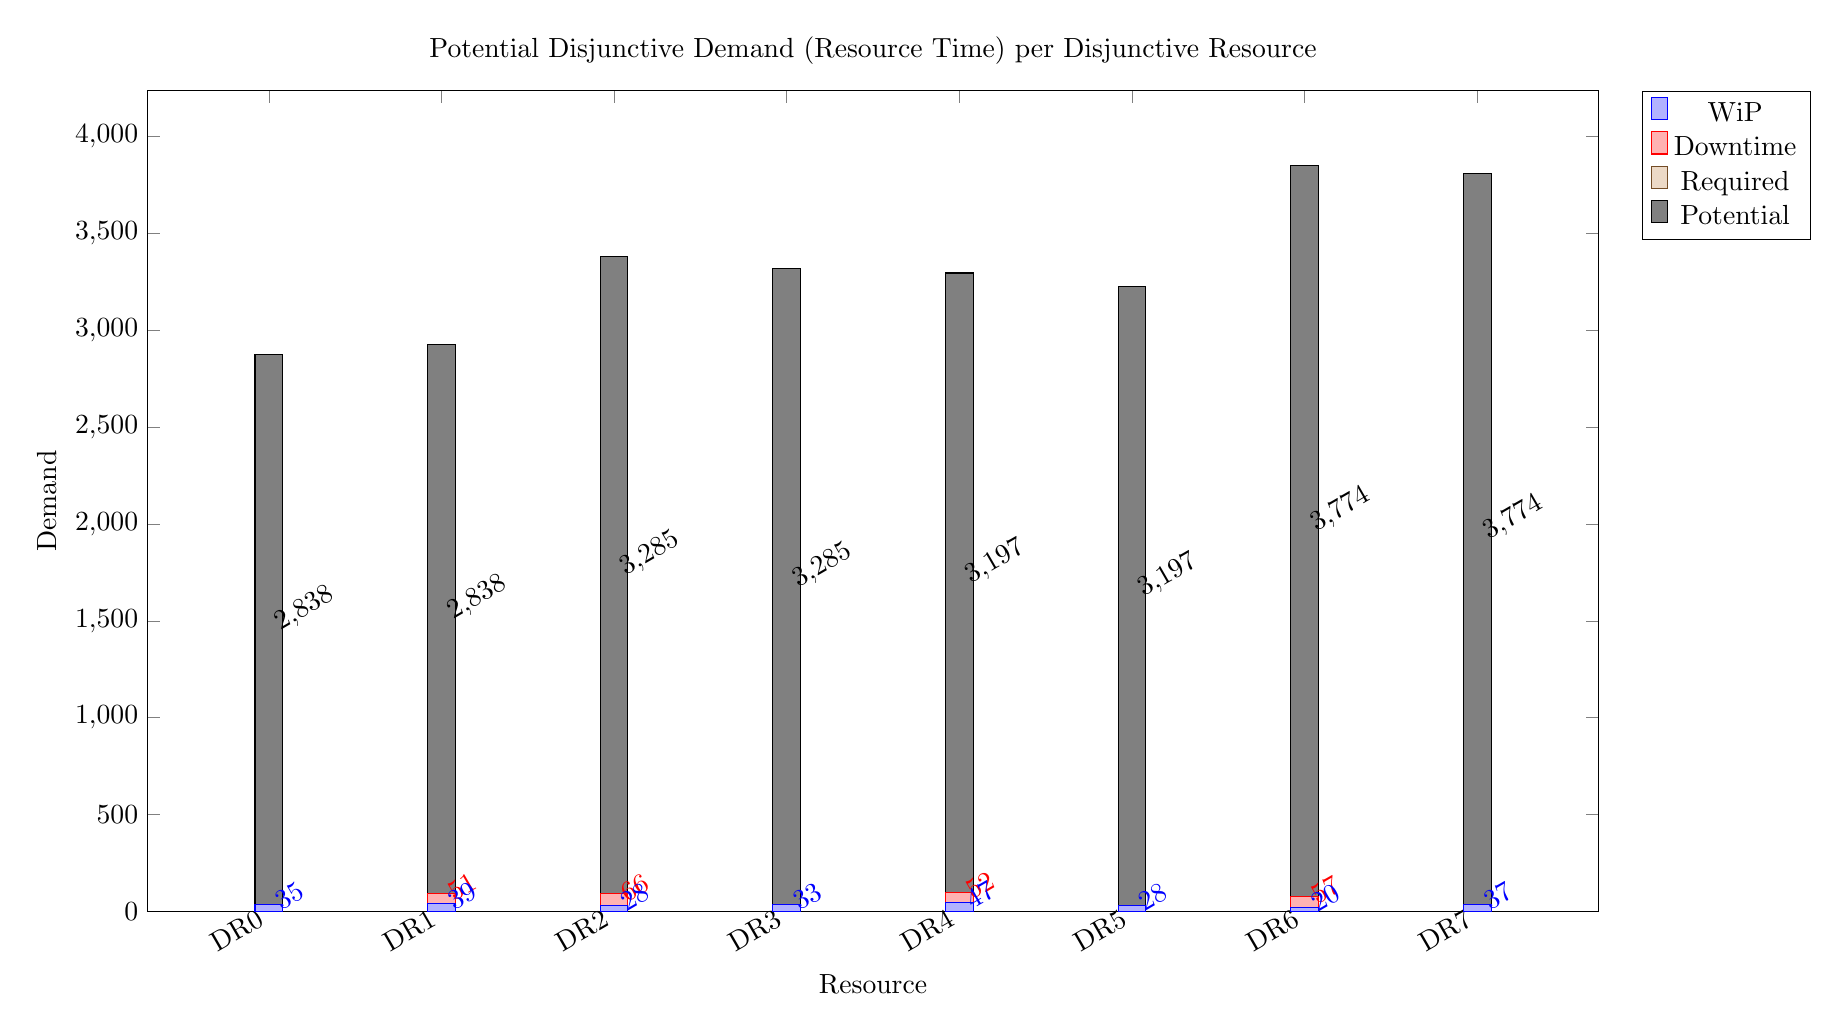
\begin{tikzpicture}
\begin{axis}[title=Potential Disjunctive Demand (Resource Time) per Disjunctive Resource,xlabel=Resource,ylabel=Demand,ymin=0,legend pos=outer north east,
width=20cm,height=12cm,ybar stacked,
symbolic x coords={DR0,DR1,DR2,DR3,DR4,DR5,DR6,DR7},
    xtick=data,nodes near coords, nodes near coords align={rotate=30),anchor=west},x tick label style={rotate=30),anchor=east}]
\addplot+[] coordinates {
(DR0,35.000000)
(DR1,39.000000)
(DR2,28.000000)
(DR3,33.000000)
(DR4,47.000000)
(DR5,28.000000)
(DR6,20.000000)
(DR7,37.000000)
};
\addplot+[] coordinates {
(DR0,0.000000)
(DR1,51.000000)
(DR2,66.000000)
(DR3,0.000000)
(DR4,52.000000)
(DR5,0.000000)
(DR6,57.000000)
(DR7,0.000000)
};
\addplot+[] coordinates {
(DR0,0.000000)
(DR1,0.000000)
(DR2,0.000000)
(DR3,0.000000)
(DR4,0.000000)
(DR5,0.000000)
(DR6,0.000000)
(DR7,0.000000)
};
\addplot+[] coordinates {
(DR0,2838.000000)
(DR1,2838.000000)
(DR2,3285.000000)
(DR3,3285.000000)
(DR4,3197.000000)
(DR5,3197.000000)
(DR6,3774.000000)
(DR7,3774.000000)
};
\legend{WiP,Downtime,Required,Potential}
\end{axis}
\end{tikzpicture}

\section{No Solutions}

\end{document}
